\section{Basic Protocol 2: Predicting ELMs in
sequences}\label{basic-protocol-2-predicting-elms-in-sequences}

One of the most useful (and used) features in ELM is the ability to
detect motifs in proteins and sequences. Given a protein's amino acid
sequence, the ``EML Predictions'' pipeline searches for occurrences of
each motif class using regular expressions, apply a set of filters to
help judging results, and to visualize resulting set of putative motifs.

In this protocol we will be viewing the manually annotated data of a
typical protein, using p53 (Uniprot ID: P53\_HUMAN/P04637) as an
example. We will cover how to find the manually annotated motifs and
instances, and how to find the motif instances, the references used to
annotate each instance, the experimental protocols used, and additional
information including relationships to biological pathways (such as KEGG
\cite{26476454}), diseases (from OMIM \cite{17357067}) and molecular
switches (in switches.ELM \cite{23550212}).

\subsection{Necessary Resources}\label{necessary-resources}

\subsubsection{Software \& Hardware}\label{software-hardware}

A modern browser such as Firefox, Chrome, or Safari. ELM is best viewed
on a laptop or desktop computer, although tablets and smartphones will
also work.

\subsection{Predicting ELM instances using data from ELM
database}\label{predicting-elm-instances-using-data-from-elm-database}

\begin{figure}[h!]
\centering
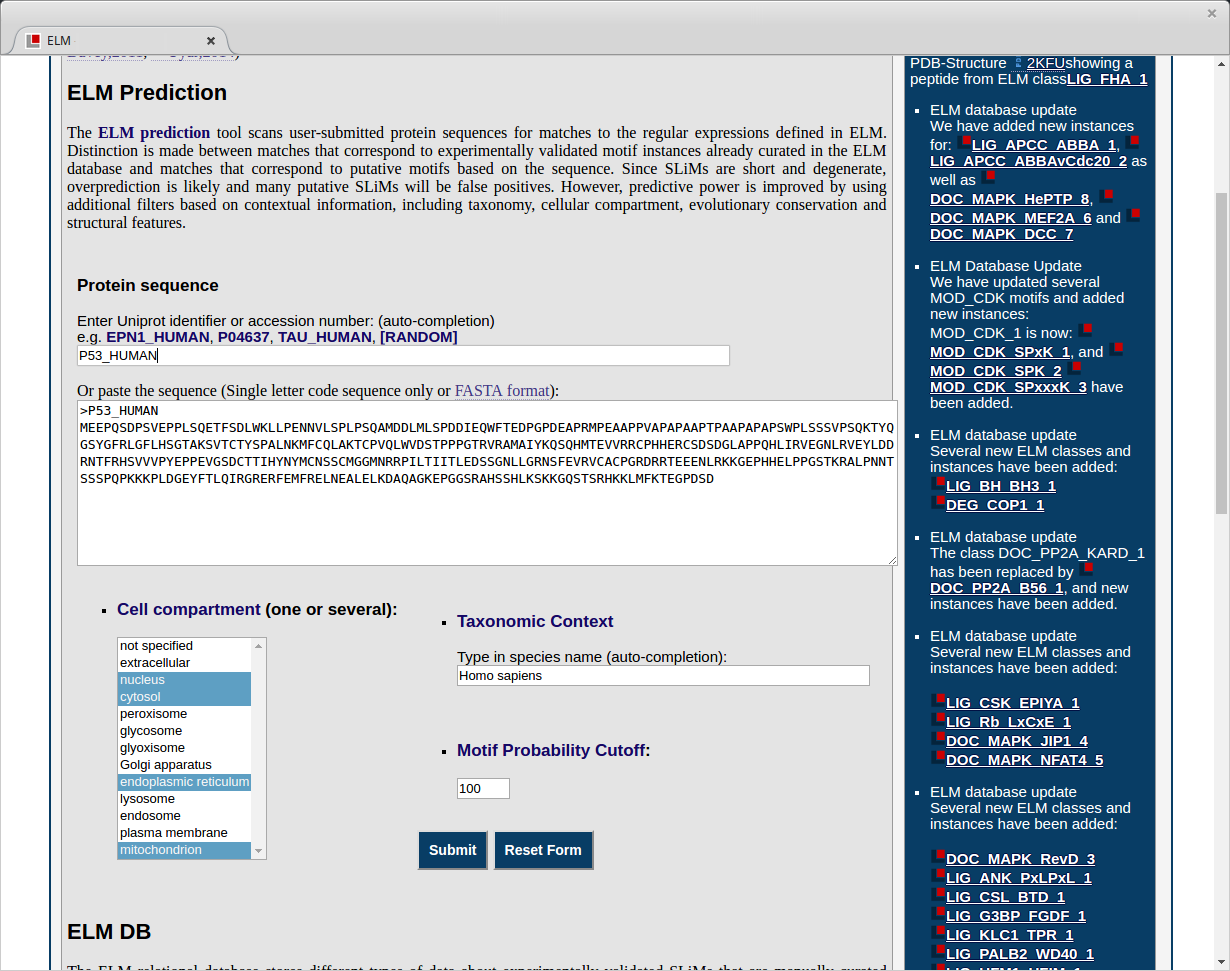
\includegraphics[width=\textwidth]{Figures/TP53_1/elm_search.png} 
\caption{
\textbf{Figure TP53-BP1-1}
The query input page for ELM for predicting motifs in a
given protein sequence.
}
\end{figure}

Step 1. Open a browser, and navigate to the ELM homepage:
http://elm.eu.org. Enter the Uniprot ID ``P53\_HUMAN'' in the search
field labelled ``Enter a uniprot identifier or accession number''. The
page should autocomplete/suggest the protein ``P53\_HUMAN / P04637 (Homo
sapiens)''. Click on this entry to confirm that we want to search for
SLiM data for this protein. Click on ``Submit'' to view the motif
instance data for p53. (Fig. TP53-BP1-1)

\sdesc{
The autocompletion mechanism queries uniprot.org for protein identifier;
if it succeeds, then additional information from uniprot will be used to
pre-populate the filter boxes. In this example, P53\_HUMAN is recognized
as a Human protein, and so ``Homo sapiens'' is automatically filled in
the ``Taxonomic Context'' field. Also, P53 has been annotated (by
Uniprot) to be localized to nucleus, cytosol, endoplasmic reticulum and
mitochondrion, so these are also automatically applied as search
criteria. The motif cutoff of ``100'' is a sufficiently high (lenient)
threshold to allow all other detected motifs to be shown.
}

step 3. Select the search criteria (optional). It is possible to limit
the results by ``cell compartment'', ``taxonomic context'' or by
changing the ``motif probability cutoff''. To restrict the search to
include SLiM's that are active in certain cellular compartments, select
one or more from the list (use the ``control'' key to select more than
one option). It is also possible to select a ``taxonomic context'' to
restrict the search to SLiMs from certain species. Start typing a
species name in the ``taxonomic context'' input field to get an
auto-completed list of species to select from. Additionaly, a ``Motif
probability cutoff'' can be used to only retain ELM classes whose
pattern probability is below the given value. For the current protocol,
leave all of these at their default values: ``not specified'', ``100''
and no ``taxonomic context''

TODO: Repeat search using stringent filters (homo sapiens, nucleus,
0.01)

\subsection{Interpreting the prediction results: Graphical
Summary}\label{interpreting-the-prediction-results-graphical-summary}

step 4. Click ``submit'' to start the searching for motifs. You will be
brought to an intermediate page indicating that your results are being
processed, and you should be redirected to the final results page within
a minute.

\sdesc{
The Results are summarized in the first figure on the results page (see
figure TP53-BP1-2). The graphical summary shows the results generated by
the ELM prediction pipeline, combined with additional filters and
information from external resources. The visualization should help you
interpreting the results and to assess whether or not a motif is present
in a sequence, as well as how likely it is to be functional based on its
structural context and evolutionary conservation. Motif instances which
are manually annotated in the database appear as red (TP) or yellow (FP)
ovals in the graphic. Blue/gray squares represent predicted motif
occurrences.
You can bookmark this page: The results are stored for a week.
}

\begin{figure}[h!]
\centering
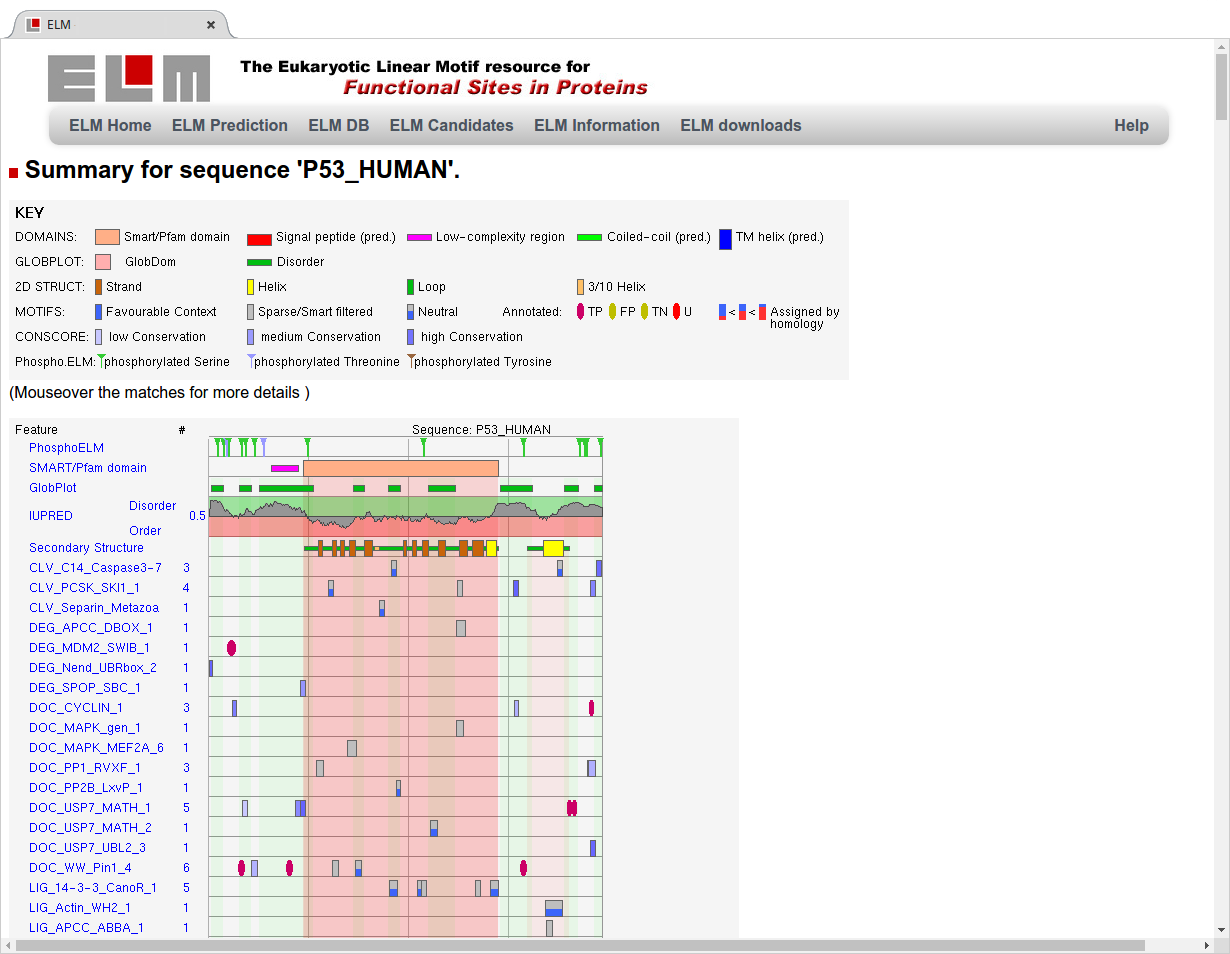
\includegraphics[width=\textwidth]{Figures/TP53_1/elm_results_summary.png} 
\caption{
TODO: caption
}
\end{figure}

\textbf{Figure TP53-BP1-2} The graphical results summary of the ELM
Prediction pipeline for ``P53\_HUMAN''. Note that not all motif
detections are shown (the image is truncated at the bottom). The top
five rows show a set of structural features. Annotated and predicted
motifs are shown as differently colored ovals/boxes.

step 6. The first row contains phosphorylation sites as retrieved from
Phospho.ELM (\cite{21062810}), and whether the phosphorylated amino acid
is a serine, threonine or tyrosine. Phospho.ELM is a database of
manually annotated phosphorylation sites obtained from scientific
publications from low and high-throughput experiments. You can follow
the link to Phospho.ELM by clicking on the phosphorylation site in the
image to get more information on individual phosphorylation sites.

\sdesc{
Phosphorylation sites are only available when the search is performed
with a protein accession (eg. \emph{not} with FASTA sequence alone) in
step XXX and there is relevant information annotated in the Phospho.ELM
database. Phosphorylation sites are relevant to interpret ELM motif
predictions when the predicted motif requires to be phosphorylated (as
in several docking and ligand binding motifs) and naturally, for the
prediction of phosphorylation motifs.
}

step 7. The second row shows SMART and Pfam domains detected by the
SMART database (\cite{9600884},\cite{25300481}, \cite{9600884}). Hover
the mouse over these domains to see their names and exact start and end
positions.

\sdesc{
In order to be functional SLiMs need to be accessble, and therefore they
are usually not found within globular domains and structured regions
(\cite{21909575}). Any SLiMs detected by the ELM prediction pipeline are
less likely to be functional, and are indicated with a red background
(see also the ``structural filter'' described in step XXX).
}

step 8. The third row shows globular and disordered regions in the
sequence as predicted by GlobPlot (\cite{12824398}). The fourth and
fifth row contains results from IUPred (\cite{15955779}), another
predictor of disordered protein regions. Protein segments with an IUPred
score above 0.5 considered to be disordered.

\sdesc{
SLiMs are typically only functional when found in intrinsically
disordered regions. Any motif occurrence detected by the ELM prediction
pipeline that falls within disordered regions are more likely to be
functional.
}

step 9. The 5th row contains information on secondary structure. The
secondary structure is predicted using a pipeline mapping motif
occurrence onto high quality reference domain structures
(\cite{19852836}). Check the graphical representation, if the output of
the secondary structure filter and the disorder predictors agree with
respect to wihch parts of the sequence are considered structured and
which disordered.

step 10. The remainder of the figure (below ``secondary structure''
output) displays predicted and annotated motif instances, overlayed by
the structural context from rows 2 and 3 (SMART domains and GlobPlot). A
blue square indicates a single motif occurence, intensity of the color
indicates the conservation of this sequence in homologous proteins.
Boxes in gray are motif occurences which have been filtered out by the
``structure filter''. Boxes that are blue \& gray are neutral (eg.
residing in structural context, but the secondary structure detected a
loop region). If the sequence is already present in the ELM database,
any motif instances that have already been annotated are shown as ovals.
Lastly, any motifs detected, which are annotated to be functional in
homologous sequences, are shown as red/blue rectangles.

TODO: EXPLAIN / SHOW ANNOTATED INSTANCES

\sdesc{
In the case that not enough homologous sequences were detected to build
an alignment, no conservation score can be calculated. Therefore all of
the motif occurences will be shown in a uniform shade of blue.
}

step 11. Place the cursor over the blue box for motif occurence
``MOD\_PLK'' at position 6-12. This motif is in a disordered region, and
has not been filtered out by the structural filter. However, its
conservation score is very low: 0.16, indicating it is not conserved in
homologous proteins.

\sdesc{
The confidence score is based on how conserved the sequence is across a
set of homolous proteins from other sequences. An full description of
the method can be found in \cite{18460207}.
}

step 12. Mouse over a gray rectangle (indicating motifs which have been
filtered out) to find out why this hit was filtered out. It shows scores
for all of the individual criteria used by the secondary structure
filter: The name of the domain, the \emph{accessibility score} ,
\emph{secondary structure score}, \emph{combined total score}, and the
associated \emph{total score P-value} (\cite{19852836}).

\begin{figure}[h!]
\centering
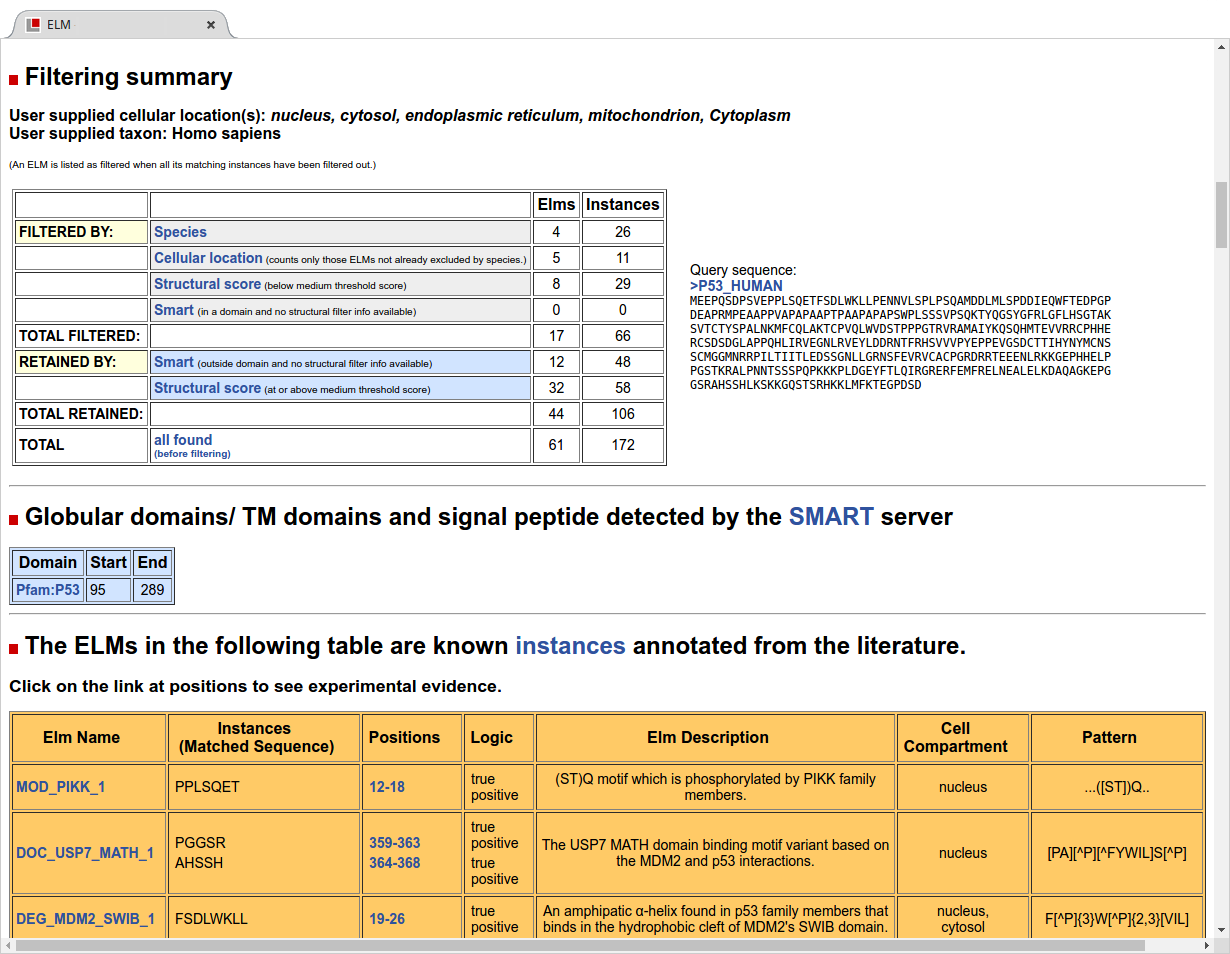
\includegraphics[width=\textwidth]{Figures/TP53_1/elm_results_alignments_filtering_domains.png}
\caption{
\textbf{Figure BACT-BP-3:} This section of the results contains
additional details of alignment of homologous proteins, filtering
results and globular domains.
}
\end{figure}

TODO: INSERT/CHANGE FIGURE/NAME

step 13. Scroll down to below the results graphic to find additional
information on the ELM Predction pipeline's results (figure BACT-BP-3).
The first section contains links to download or view the multiple
sequence alignments of homologous proteins used to calculate the
conservation score. Click on the link ``Click here to enable the
multiple sequence alignment viewer'' to open the alignment in Jalview
(note: this requires the Java browser plugin, which might not be
available on some browsers). Alternatively you can also download the
``alignment'', ``conservation features'' and ``phosphosite features''
files separately to view on a desktop (non-browser) installation of
Jalview (\cite{19151095}).

\sdesc{
The search for possible homologs is performed against the UniRef90
database, a dataset of protein sequences with less than 90 percent
identity between any two of them (\cite{17379688}). It is also possible
that the BLAST results are not finished when the results page is shown:
We suggest to refresh the page if you see the message ``Either not
enough data available to calculate a sequence alignment or the
calculations haven't finished yet''. In some cases it is also possible
that no homologs will be detected. If you have refreshed the page after
waiting for more than 3 minutes, this is most likely the case.
}

step 14. Scroll down to the section titled ``Filtering Summary'' to view
some statistics about how many motifs and instances were filtered out
(figure TP53-BP1-2). The first two lines contain information on whether
and which filters were applied in step XXX of this protocol. The next
two lines (SMART \& Structural score) show how many motifs and instances
were removed by the SMART and Secondary structure filters. The
``Retained by'' section shows how many motif hits were not filtered out
by the ``Smart'' or ``Structural Score'' filter. In this example a total
of XXX instances (of XXX different motifs were identified), of which XXX
instances (and XXX motifs) were filtered out as they occured in a SMART
domain.

\sdesc{
Note that the graphical summary above does not contain sequences
filtered out by the ``cell compartment'' and ``taxonomic context''
filters (in step XXX). However those filtered out by the SMART and
Structural scores are shown in the graphic above (as gray rectangles).
If any ``cell compartment'' or ``taxonomic context'' filters are
selected in step XXX, the number of motifs and instances are also shown
in this table.
}

\begin{figure}[h!]
\centering
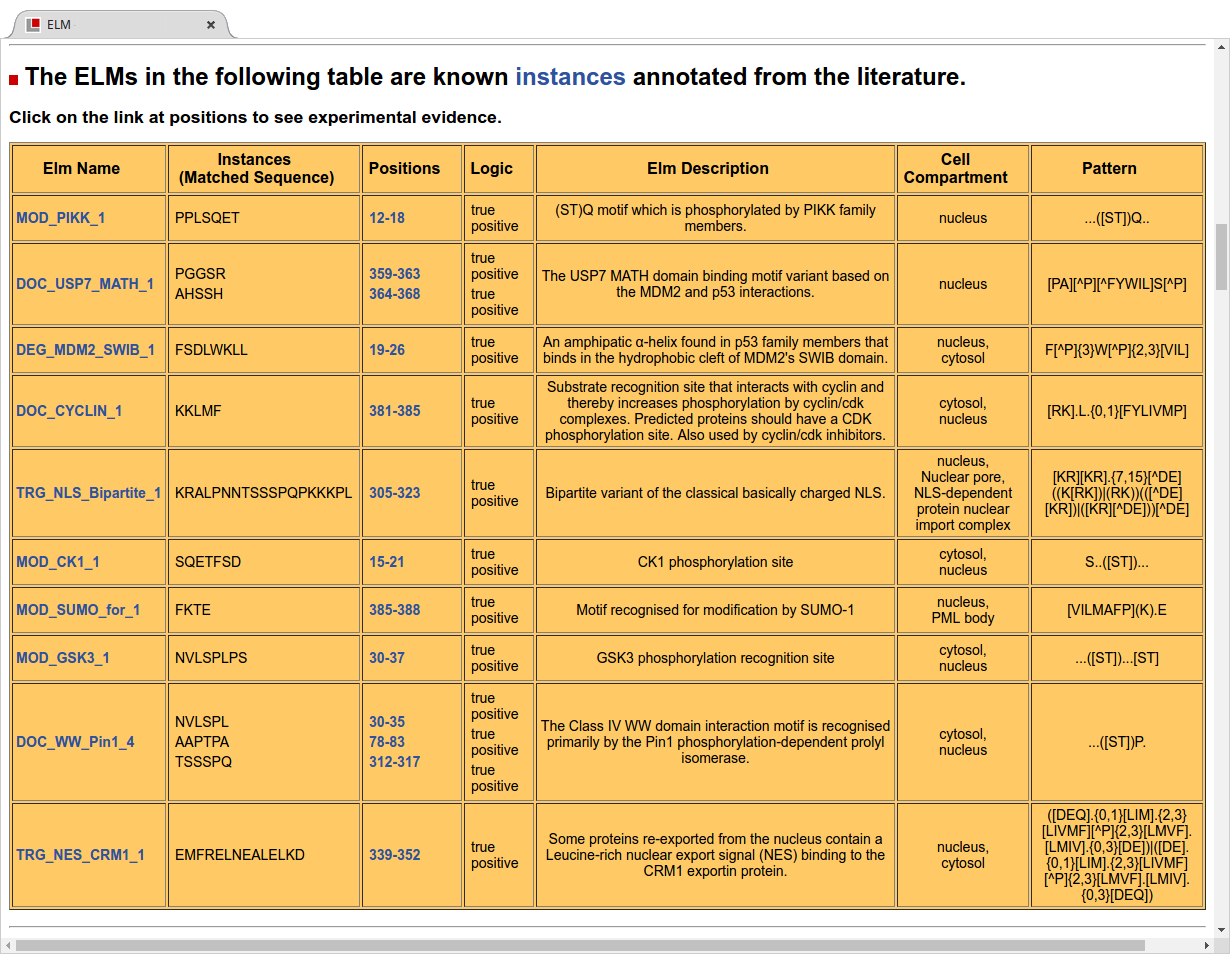
\includegraphics[width=\textwidth]{Figures/TP53_1/elm_results_known.png} 
\caption{
\textbf{Figure TP53-BP1-3}
}
\end{figure}

Step 15. On the results page, scroll down to the heading: ``The ELMs in
the following table are known instances annotated from the literature''
(Fig TP53-BP1-3). This table has details of SLiMs which have been
manually annotated in the ELM database. The columns show each motif
name, the sequence(s) that matched the motif as well as their starting
and ending positions and the logic of the annotation followed by a short
description of each motif, to which cell compartments its has been
associated, and finally the regular expression of the motif.

\sdesc{
The ``Logic'' column indicates whether this motif is an example of a
functional (True Positive, TP) or non-functional (False Positive, FP)
motif. A TP instance is an instance annotated with experimental evidence
showing this instance to be functional, whereas a FP is an instance with
experimental evidence hinting at a function, but after careful
inspection our annotators believe this instance to be non-functional.
There are only rare cases of a true negative (TN) instance, which is an
annotated instance where experiments have shown it to be non-functional.
}

TODO: INSERT/CHANGE FIGURE/NAME

step 16. Scroll down to the section with the header ``Globular domains/
TM domains and signal peptide detected by the SMART server'' (Figure
BACT-BP-3). This section contains information on which domains were
detected by the SMART server, and their positions. Clicking on their
names will bring you to the SMART entry for that domain on the SMART
homepage.

TODO: INSERT/CHANGE FIGURE/NAME

\begin{figure}[h!]
\centering
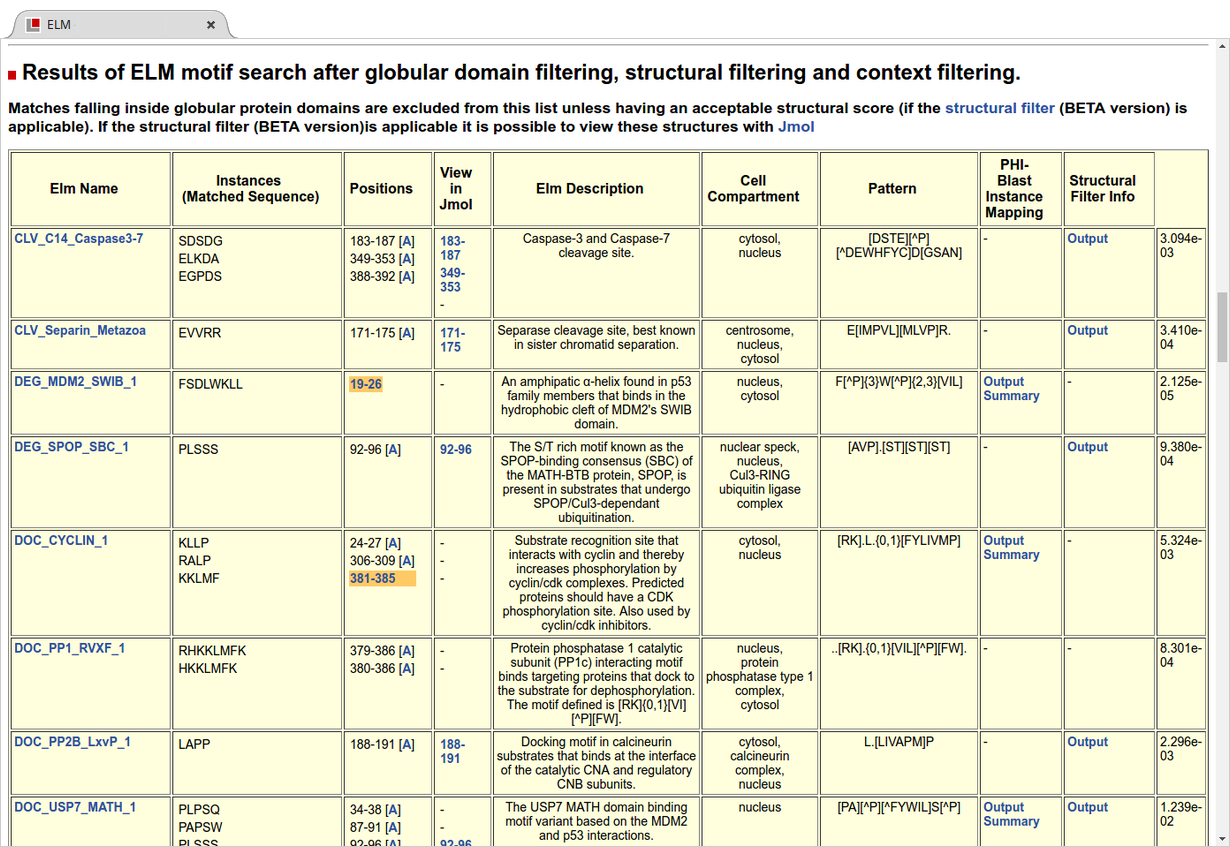
\includegraphics[width=\textwidth]{Figures/TP53_1/elm_results_motifs.png}
\caption{
\textbf{Figure BACT-BP-7:} This table contains the list of motifs
detected in the sequence (only the top part of the table is shown).
}
\end{figure}

TODO: INSERT/CHANGE FIGURE/NAME

step 17. Scroll further down to the section title ``Results of ELM motif
search after globular domain filtering, structural filtering and context
filtering'' to obtain an overview of all of the motifs and motif
instances detected (Figure BACT-BP-7). Each row also contains
information on the Motif name, the matching peptide sequence and its
position. Additional information is shown about the ELM, cell
compartment and its regular expression. If the motif was detected in a
homologue, the column called ``PHI-Blast Instance mapping'' contains
links to the Sequence alignment of the homologous protein, and a summary
of the ELM instance mapper output. If a motif instance has been filtered
out due to Structural criteria (SMART or Structure), this column
contains a link to a page with details on how individual criteria that
make up this filter. The last column contains information on the
Probability filter: the probability reflects the chance to observe this
motif in any random amino acid sequence.

TODO: INSERT/CHANGE FIGURE/NAME

\begin{figure}[h!]
\centering
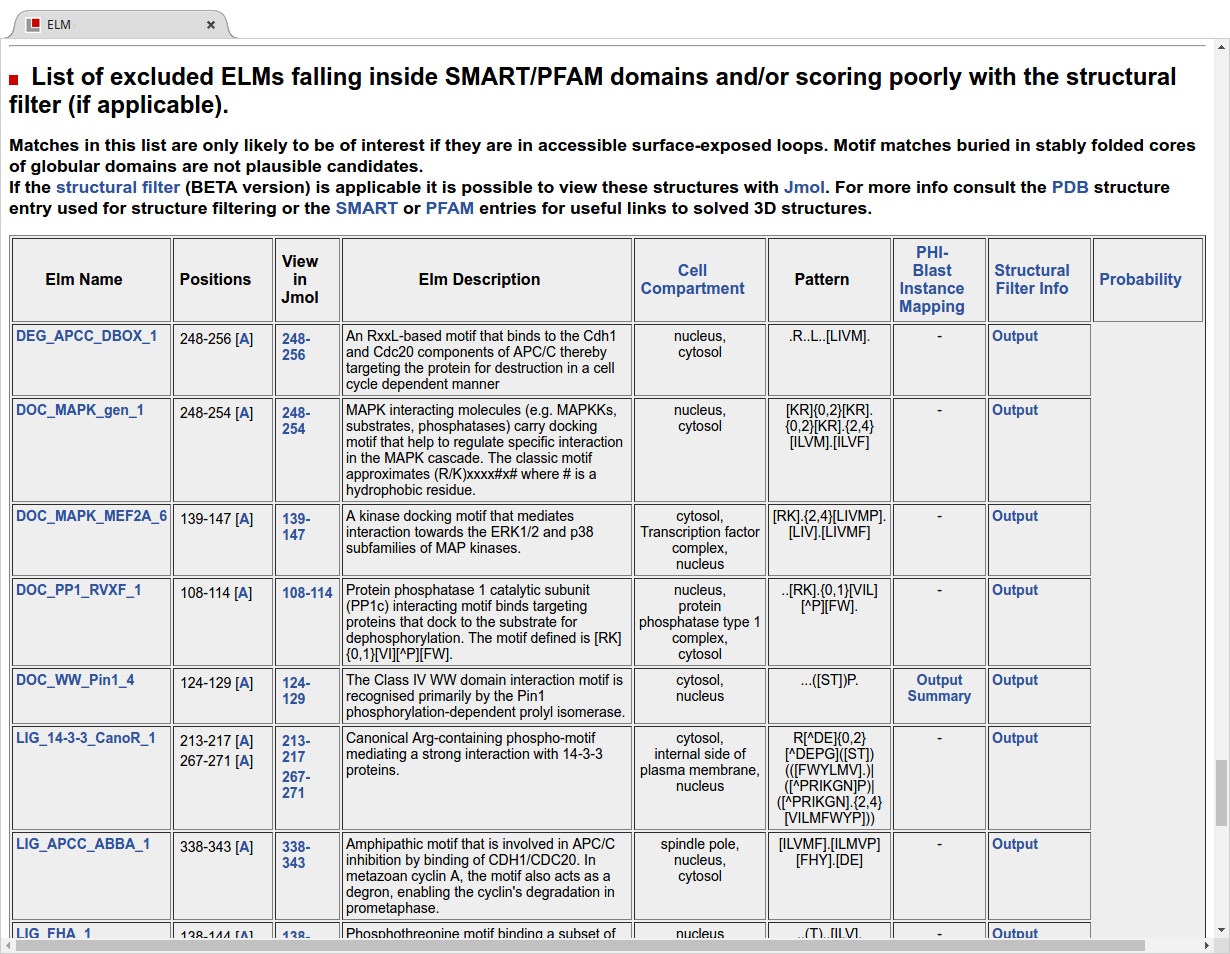
\includegraphics[width=\textwidth]{Figures/TP53_1/elm_results_motifs_filtered.png}
\caption{
\textbf{Figure BACT-BP-8:} This table contains the list of motifs
detected in the sequence (only the top part of the table is shown) which
were excluded due to structural filters.
}
\end{figure}

TODO: INSERT/CHANGE FIGURE/NAME

step 18. Scroll further down to the heading ``List of excluded ELMs
falling inside SMART/PFAM domains and/or scoring poorly with the
structural filter (if applicable).'' (Figure BACT-BP-8). This table is
(almost) identical to the one above, but shows motif instances which
were rejected by the Structural filter or SMART filter.

